\documentclass[letterpaper]{article}

% NIPS header
\usepackage{nips10submit_e,times} 
\usepackage{helvet} 
\usepackage{courier}
\usepackage{url}

% fancy symbols
\usepackage{amsmath}
\usepackage{amsthm}
\usepackage{amssymb}
% \usepackage{natbib}
\usepackage{graphicx}
\usepackage{subfigure,fullpage}

\newtheorem{thm}{Theorem}
\newtheorem{lemma}{Lemma}
\newtheorem{definition}{Definition}
\newtheorem{question}{Question}

\title{Learning To Classify Review Usefulness}
\author{Ertan Dogrultan, Cesar Romero, Paul Wais\\
Computer Science Department \\
University of California, Los Angeles\\
Los Angeles, California 90095\\
\texttt{\{ertan,romero\}@cs.ucla.edu, pwais@ucla.edu}}

\nipsfinalcopy

\begin{document}
\maketitle
\begin{abstract}
  In this work, we study the learning task of predicting if a product or 
  business review will receive ``useful'' votes.  We study a corpus of
  2 million Amazon reviews and 15,000 Yelp reviews annotated
  with voting information.  To predict ``usefulness'', we study over a dozen 
  novel text and contextual features inspired by previous work on 
  sentiment analysis.  Furthermore, we study the task of domain adaptation,
  where we attempt to devise a classifier that performs well on Yelp data
  when only small amount of Yelp but large amount of Amazon training data
  is available.
\end{abstract}

\section{Introduction}
\label{sec:introduction}

Review-based social networks empower users to make informed purchasing
decisions.  Amazon and Yelp are two such networks that feature
millions of user-contributed consumer product and local business
reviews.  A central challenge facing these networks is the task of
quickly connecting users with useful review content.  For example,
many products and businesses on these websites feature hundreds of
user-contributed reviews, so the site must automatically identify and
spotlight the most relevant of these reviews in order to keep viewers
engaged.  In order to surface the best content, many review-based
social networks employ a user voting mechanism that enables viewers to
anonymously vote a review as ``useful.''  Unfortunately, though many
viewers do make use of this feature, most reviews do not receive votes
(see Figure \ref{fig:vote-histos}).  In this work, we study applying modern
machine learning algorithms to textual review features in order to
automatically predict if a review will receive ``useful'' votes.

An additional problem facing these networks is to spotlight quality
content in emerging areas of the site.  For example, when a social
network extends to a new foreign language or expands to a new product
domain, the network might purchase or otherwise establish seed review
content, but these reviews will not feature viewer-contributed votes.
In this setting, it is useful to adapt a model trained on existing
user votes to spotlight new content that viewers will find useful.  In
this work, we study how to fulfill this task using a domain adaptation
technique \cite{JennLearnDiffDomains}.

The remainder of this paper proceeds as follows: first we describe the novel 
features we use and contrast them with related work in sentiment 
classification.  Next, we present the results of applying traditional 
supervised learning algorithms to learn to predict the ``usefulness'' of 
reviews from Amazon and Yelp.  Next, we investigate the problem of domain 
adaptation by training a linear SVM on a preponderance of Amazon review data 
and a small sample data.  Despite spending considerable effort on feature 
engineering and classifier tuning, we observe high error rates for both of the 
aforementioned experiments.  We find that the problem of predicting usefulness 
is harder than the related problem of sentiment classification.  We conclude 
with suggestions for additional features and experiments that may result in 
a more accurate model.

\begin{figure}[h]
    \label{fig:vote-histos}
	\centering
	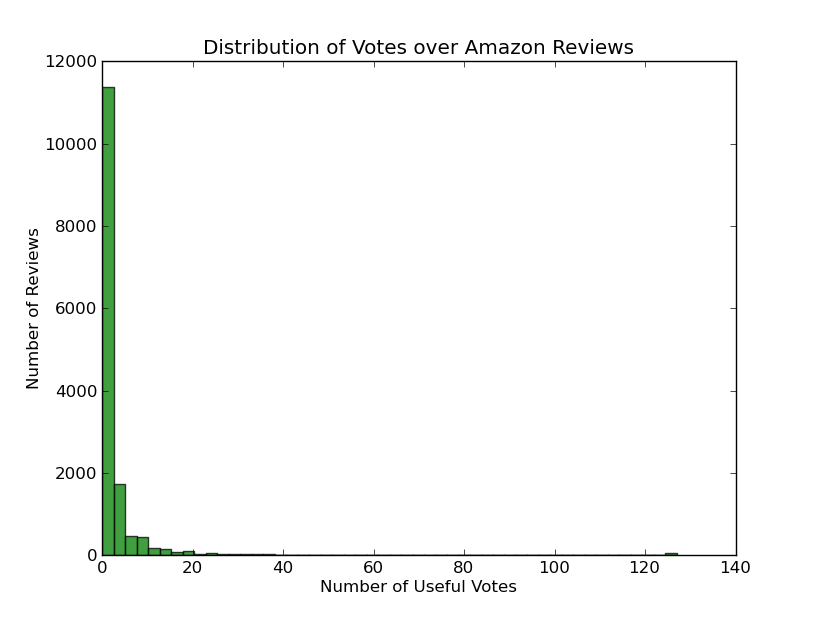
\includegraphics[width=0.30\linewidth]{amz_histo}
    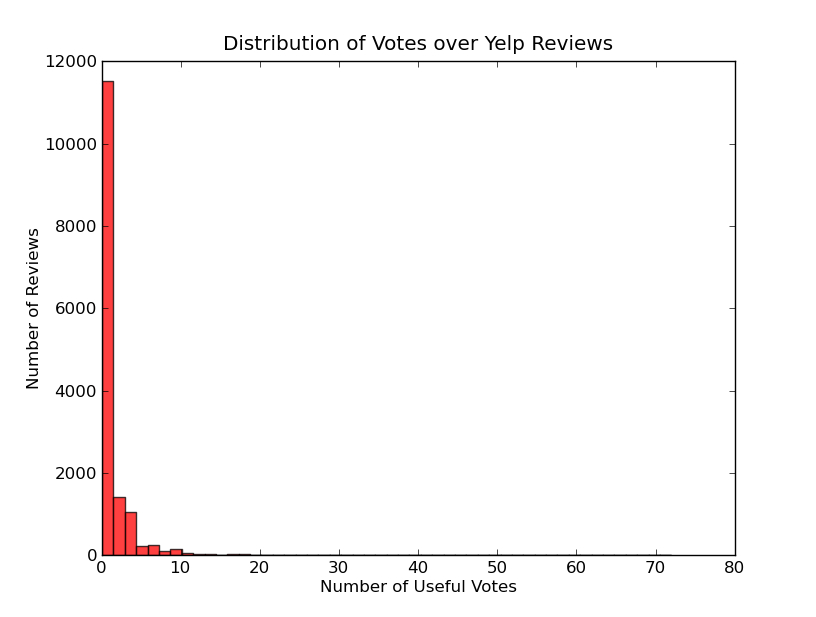
\includegraphics[width=0.30\linewidth]{yelp_histo}
	\caption{Histograms of votes in samples of 15,000 Amazon and Yelp reviews.
    Most reviews have zero votes.}
\end{figure}

\section{Related Work}
Our approach builds on related work in sentiment classification that seeks to 
use review text to predict the ratings of users' reviews.  Pang et al 
\cite{PangSentimentClassification} apply several supervised machine learning 
algorithms to movie reviews, hypothesizing that algorithms will learn to
identify a small set of words that indicate sentiment.  Their model represents 
reviews as sparse vectors in a high-dimensional space where the $i$th component 
of an input vector $\vec{x}$ indicates the count or presence for a single 
unigram or bigram.  Their experiments show that standard, un-tuned machine 
learning algorithms are capable of separating classes of positive- and 
negative-rated reviews with over $80\%$ accuracy.  

Since usefulness is independent of sentiment (i.e. negative reviews are often
very useful), we choose to study a slightly different set of features that
indicate strong argument. In the next section, we briefly describe and justify
our chosen features.

\section{Feature Extraction and Defining Labels}
\label{sec:features}

\subsection{Word Frequencies and Counts}
In an attempt to measure user effort, we measure as features the number of 
words in the review, the mean number of words per sentence, and the total 
number of sentences in the review. Additionally, we count the number of URLs, 
since users who include links tend to put more effort into reviews.

Furthermore, we measure the frequencies of several different categories of 
words and n-grams.  In particular, these categories include sets of words that
are indicative of time, space, comparisons, contrasts, summarizations,
suggestions, and emphasis.  For instance, comparison words are \emph{similarly,
likewise,} etc., and contrast n-grams are \emph{but, however, nevertheless, 
in spite of,} etc. We also measure frequencies of SAT and GRE words.  We 
normalize each count by dividing by the review's word count.

\subsection{Grammatical, Spelling, and Stylistic Errors}
Poor style and grammar often distracts users.  We count the number of grammar 
and spelling errors by feeding each review into Microsoft Word. We also 
consider the number of capitalization mistakes and words with all capital 
letters. As before, we normalize these feature values by dividing
counts by review word count.

\subsection{Emphatic Word Score}
Emphatic reviews are often more useful than neutral opinions.  We define a 
textual feature that measures sentiment strength independent of positivity
using empirical sentiment measures from The Study on Affective Norms from 
English Words (ANEW)\cite{BradleyANEW}.\footnote{In particular, we used this PDF 
available freely online \url{http://dionysus.psych.wisc.edu/methods/Stim/ANEW/ANEW.pdf}.}
Dodds et al \cite{DoddsANEWPaper} propose an effective sentiment scoring model 
that interprets the ANEW study's ``valence'' score (a real number in $[1,10]$) 
as a measure of sentiment.  (For example, in the ANEW study, ``triumph'' has a 
valence score of $8.87$, while ``hostage'' has a score of $2.20$).  Dodds et al 
propose scoring text using the weighted sum 
\[
    \frac{\sum^n_{i=0} v_i f_i}{\sum^n_{i=0} f_i}
\]
where $v_i$ is the valence and $f_i$ is the frequency of the $i$th distinct
word, respectively.  They find that this score effectively differentiates
positive and negative sentiment text across several domains.  We include
this scoring mechanism as one of our features.

\subsection{Product/Service Related Features}
The price of a product or business might impact the visibility of reviews
since expensive products and businesses are relatively sparse.  We include
as a feature the price of the product or business expressed as an integer 
between 1 (cheap) and 4 (expensive).

\subsection{Defining Usefulness Labels}
We experimented with several different ways of mapping raw useful vote
counts to binary labels.  In early experiments, we computed a histogram
of all vote counts and used a $50^{th}$ percentile cutoff to define binary
labels. In other words, if the number of positive votes
for a review is above the $50^{th}$ percentile, we labeled it as
useful. We observed that this label definition resulted in very low
classification accuracy.  In an effort to eliminate weak examples of 
each class from the training data, we redefined labels such that a review as
useful if its positive count is in the $75^{th}$ percentile or above
and not useful if they are in the $5^{th}$ percentile or below.  We found that
this label definition dramatically improved our accuracy.


\section{Single Domain Experiments}
\label{sec:single_domain}  
In this section we discuss the results of running several experiments using 
the open-source data mining framework WEKA~\cite{weka}.  We present the results 
for three algorithms: Support Vector Machines, Adaboost and Naive Bayes with 
two different feature encodings.

In the first encoding, we each input vector consists of a list of the feature
values described in Section~\ref{sec:features}. We refer to this encoding as 
\emph{dense}.

Our second feature encoding aims to follow the work of Pang et al 
\cite{PangSentimentClassification} and utilizes a higher-dimensional space. In 
place of the word frequency features described in Section \ref{sec:features}, 
we store the count of each specific word or n-gram in distinct components of 
the input vector.  We refer to this encoding as \emph{sparse}. The
main motivation behind the sparse features is increasing the dimension
for classification. This can be useful for SVMs and Adaboost
algorithms.

\begin{table}[ht]
\centering
\begin{tabular}{c | c c | c c}
 & \multicolumn{2}{|c|}{Amazon} & \multicolumn{2}{|c}{Yelp} \\
\hline
Algorithm & Training Err. & Cross Val.(5 fold) & Training Err. & Cross Val.(5 fold)\\
\hline
SVM (Linear) 		& $71.0316\%$ & $70.8\%$ & $70.305\%$ & $70.2879\%$\\
SVM (Polynomial) 	& $73.1041\%$ & $72.4316\%$ & --- & $71.3417\%$\\
SVM (Gaussian) 		& $66.053\%$ & $66.053\%$ & $68.7971\%$ & $69.1484\%$\\
AdaBoost 			& $71.0316\%$ & $72.201\%$ & $71.3588\%$ & $70.3136\%$\\ 
Naive Bayes 		& $70.719\%$ & $70.6727\%$ & $66.9037\%$ & $66.5781\%$\\ 
\end{tabular}
\caption{Accuracy using dense feature encoding}
\label{tab:dense}
\end{table}


\begin{table}[ht]
\centering
\begin{tabular}{c | c c | c c}
 & \multicolumn{2}{|c|}{Amazon} & \multicolumn{2}{|c}{Yelp} \\
\hline
Algorithm & Training Err. & Cross Val.(5 fold) & Training Err. & Cross Val.(5 fold)\\
\hline
SVM (Linear) 		& --- & $72.2357\%$ 		& --- & $70.0163\%$\\
SVM (Polynomial) 	& --- & $66.053\%$ 		& --- & $70.0592\%$\\
SVM (Gaussian) 		& --- & $72.4673\%$ 		& --- & $71.1062\%$\\
AdaBoost 			& $71.68\%$   & $70.7769\%$ & $71.2091\%$ & $70.7286\%$\\ 
Naive Bayes 		& $76.8091\%$ & $73.0346\%$ & $77.1733\%$ & $67.9567\%$\\ 
\end{tabular}
\caption{Accuracy using sparse feature encoding}
\label{tab:sparse}
\end{table}

Tables~\ref{tab:dense} and~\ref{tab:sparse} show the results for this
set of experiments. First, we want to focus on the performance
improvement Naive Bayes shows when switching to the sparse encoding. The main 
problem with this classifier is believed to be the lack of low entropy feature
distributions~\cite{naivebayes}. We believe that the unrealistic
assumption of conditional independence between the features hurts the
accuracy significantly. Moreover, we note that there are overlaps
among the word categories described in Section \ref{sec:features}; not only 
in the actual words but in meanings as well. Therefore, switching to the sparse 
encoding removes dependencies between features that could normally reduce the
performance of Naive Bayes. The Tables show how the accuracy increases
from $70\%$ to $76\%$ for Amazon and from $66\%$ to $77\%$ for Yelp.

In many applications, the Adaboost algorithm tends to have low training
error, so we investigated the performance of Adaboost more closely. We
look at our weak classifiers and the corresponding errors,
$\epsilon_t$. At each step, the weak classifier $h_t(x)$ having the
minimum error on the weighted samples is chosen greedily. The 
weak classifier chosen at step $t=0$ (which is usually the number of words 
in the text with a certain threshold) has $\epsilon_t \approx 0.34$. However,
most other classifiers have very high error rates, with $\epsilon_t \approx
0.4999999$. As we looked at the histograms of feature distributions over the 
labeled samples, we observed that they were either very sparse (i.e. few
buckets have reviews in them) or the histograms overlapped. As we
extract a weak classifier that corresponds to a feature, the threshold
cannot classify significantly better than random decision due to this
overlap. Keeping this empirical observation in mind, we revisit the
upper bound for the training error for
Adaboost~\cite{adaboost,adaboost2}. We have
\[
err(H) \leq e^{-2\gamma^2 T}
\]
where $\forall t$, $\gamma_t \geq \gamma $ and $\gamma > 0$. In our
experiments, we witness an arbitrarily small $\gamma$. We believe that
this explains the poor performance of the strong classifier.

Looking at the performance of Adaboost and linear SVMs with dense and
sparse encodings, we observe similar accuracies for both Amazon and
Yelp data. We believe that the class distribution of useful reviews has 
a significant effect on the accuracy. This conclusion originates from 
the observation of ``bad'' confusion matrices ($CM$) for the classifiers. 
Indeed, as we look at the confusion matrices of both algorithms on the 
Amazon data set in Equation~\ref{eq:confusion}, we do not see the desired 
dominant diagonal.
\begin{equation}
\label{eq:confusion}
CM_{Adaboost} = \left(
\begin{matrix}
4551 & 1154\\
1247 & 1685
\end{matrix}
\right)
\qquad
CM_{linearSVM} = \left(
\begin{matrix}
5486 & 219\\
2303 & 629
\end{matrix}
\right)
\end{equation}
As we investigate further by changing the labeling for the reviews, we
see its effect on class distributions directly in the confusion
matrices. We compare the behavior of Adaboost and linear SVM by
looking at the specific examples represented in these confusion
matrices. Equation~(\ref{eq:confusion}) shows how Adaboost is
performing better than linear SVMs in this aspect.

\section{Adapting From Amazon to Yelp Reviews}
\label{sec:background}

In this section we study the task of training a classifier on an abundance of
Amazon data (i.e. a source domain $S$) and a small amount of Yelp data (i.e 
a target domain $T$) in order to predict the usefulness
of Yelp reviews. We discuss results of following the procedure of Ben-David 
et al \emph{domain adaptation}~\cite{JennLearnDiffDomains}.  To be able to 
estimate a bound on the error, two important concepts are taken into account: 
the divergence between unlabeled data in both domains and the $\alpha$ error,
which expresses a weighted tradeoff between source and target training error.
For the purpose of this experiment, we use a linear SVM as our classifier.

In this setting, we calculate the divergence between two domains by
training a classifier on ``unlabeled'' data. In particular, the error of 
this classifier is used to estimate the domain divergence.

Given the two domains we are interesting in learning a hypothesis $h$
that minimizes an empirical error that combines both domains. This is
precisely the $\alpha$-error defined as $\alpha \hat
\epsilon_T(h)+(1-\alpha)\hat \epsilon_S(h)$, where $\hat \epsilon_S$
and $\hat \epsilon_T$ are the source and target errors,
respectively.  We express the target error bound as a function of alpha in 
Equation~(\ref{eq:alphaerror}), where $\zeta(U_S,U_T)$ is the
empirical divergence and $\beta$ is the fraction of training from the target
domain.

\begin{equation}
  \label{eq:alphaerror}
  f(\alpha)=\sqrt{\frac{C}{m}\left(\frac{\alpha^2}{\beta} + \frac{(1-\alpha)^2}{1-\beta}\right)}+(1-\alpha)\zeta(U_S,U_T)
\end{equation}

\begin{figure}[h]
	\centering
	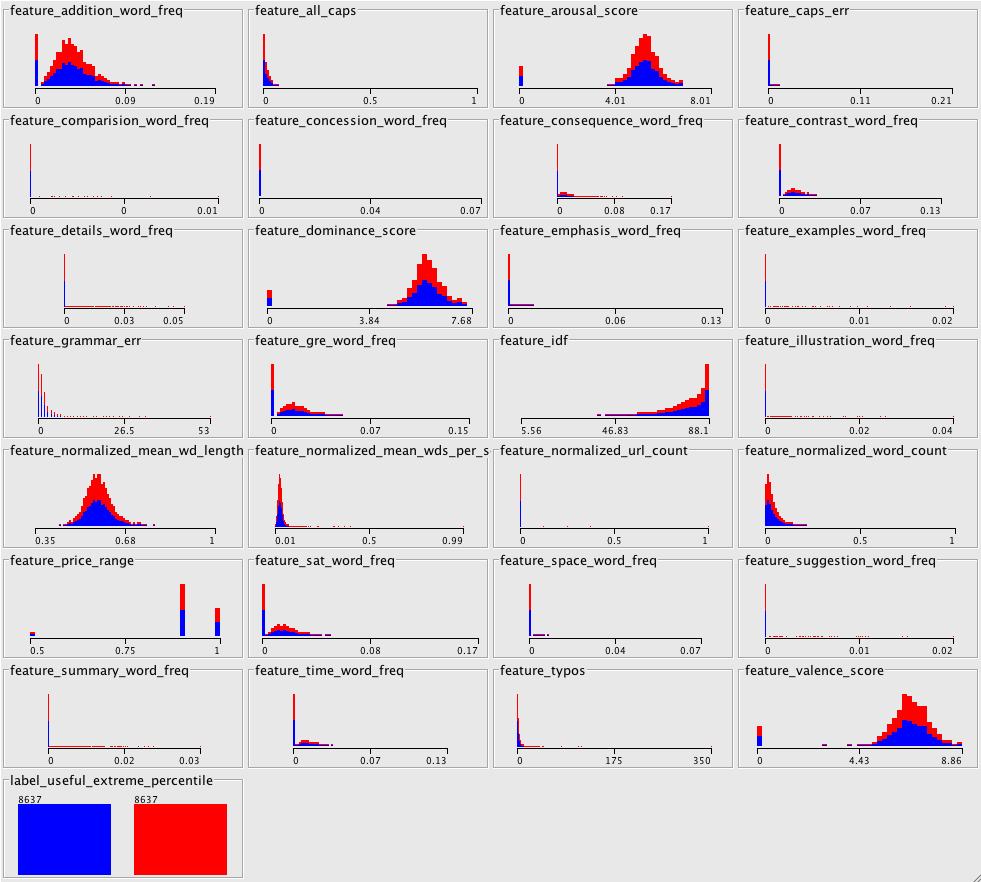
\includegraphics[width=0.65\linewidth]{adaptation_unlabeled_features}
	\caption{Feature distributions for the unlabeled data sets $U_{\textrm{A}}$ and $U_{\textrm{Y}}$.  
	Blue indicates Amazon data feature values and red indicates Yelp feature values.}
      \label{fig:dist}
\end{figure}

\subsection{Experiments}
\label{sec:domain-adaptation}

We estimate the divergence $\zeta(U_S,U_T)$ as described in the
previous section combining 10,000 examples from each
domain. Figure~\ref{fig:dist} shows the feature distributions for both
domains. The large overlap for each feature suggests that the domains are 
very similar, which would imply a low divergence. However, our 
classifier-induced divergence was very close to one in practice.

We performed two sets of experiments. First, we fix the number of
examples from the source domain constant $m_s=2500$, and we vary the
examples from the target distribution $m_t \in \{250, 500, 1000,
2000\}$. Then, we fix $m_t=2500$ constant and we vary $m_s$ in the
same way. 

Figure~\ref{fig:domain-adaptation} shows the results of both
experiments. The left column corresponds to the first experiments where
$m_S$ is fixed; the right column to the experiments where $m_T$ is
fixed. Top row shows a theoretical bound on the error given by
Equation~(\ref{eq:alphaerror}) and the bottom row shows experimental
results.

\begin{figure}[ht]
  \centering
  \subfigure[$\zeta(U_S, U_T)=1, m_S=2500$]
  {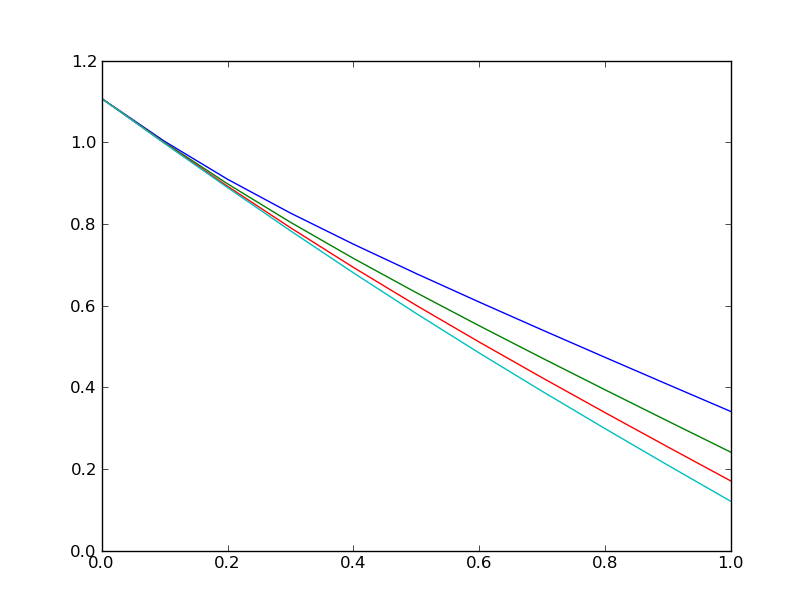
\includegraphics[scale=.3]{adaptation_bound_1_S}}
  \subfigure[$\zeta(U_S, U_T)=1, m_T=2500$]
  {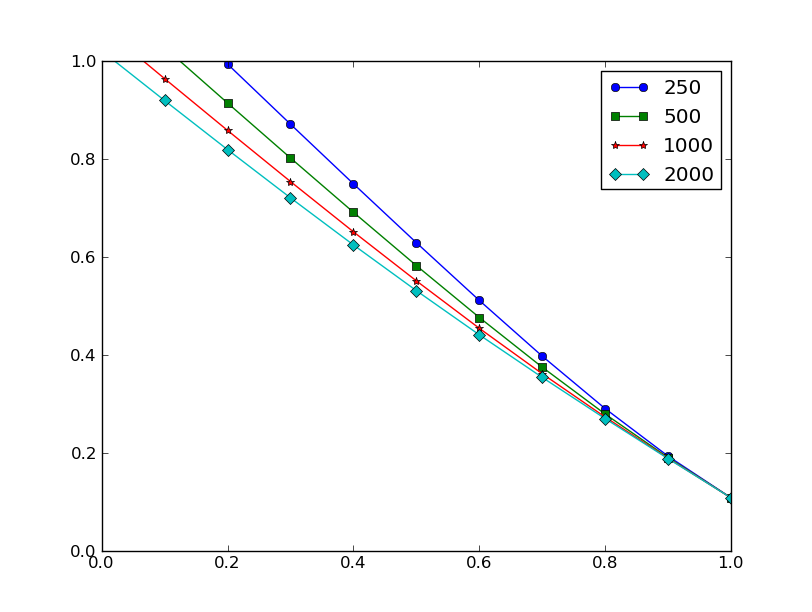
\includegraphics[scale=.3]{adaptation_bound_1_T}}
  \subfigure%[$\zeta(U_S, U_T)=1, m_S=2500$]
  {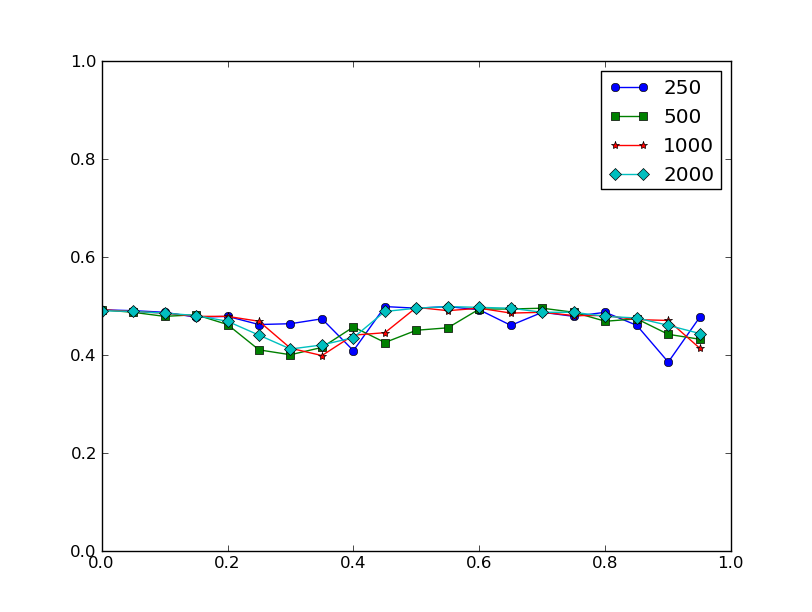
\includegraphics[scale=.3]{adaptation_err_S}}
  \subfigure%[$\zeta(U_S, U_T)=1, m_T=2500$]
  {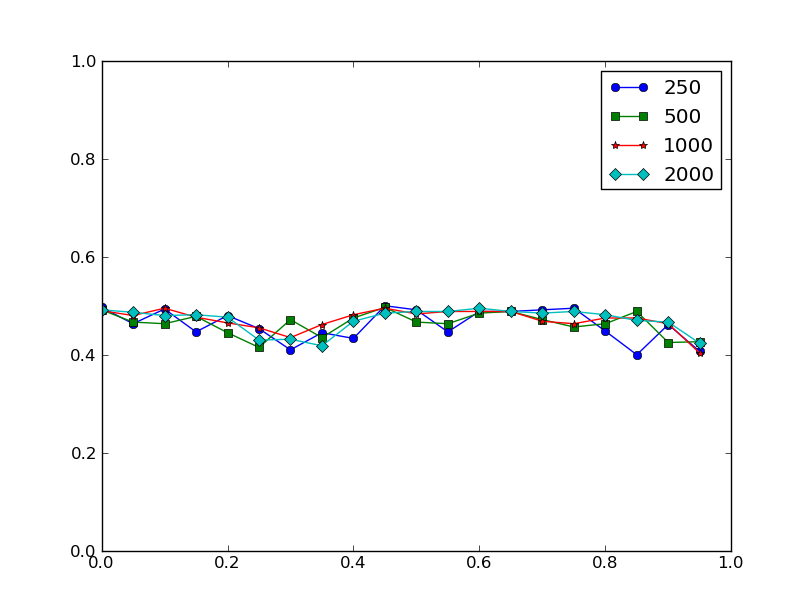
\includegraphics[scale=.3]{adaptation_err_T}}
  \caption{Domain adaptation experiments. The $\alpha$-error is shown as a function of $\alpha$ for different combinations of source and target examples.}
  \label{fig:domain-adaptation}
\end{figure}

\section{Future work and Conclusion}
\label{sec:future-work}

Looking at the performances of the algorithms, we observe Adaboost and
linear SVM have similar accuracies on most of the various experiment
instances. As stated in Section \ref{sec:single_domain} one of the
obvious differences is the quality of the confusion matrices. We would
like to investigate the incorrectly classified examples for each
algorithm and come up with an explanation related to what it is
minimizing for classification.  Furthermore, we would like to give a
more rigorous explanation on why Naive Bayes classifier has a
dominating accuracy in sparse feature encoding by comparing the
objective functions of our algorithms.

For domain adaptation part, we would like to see how well the
classifier performs when the distance between the target and source
distribution varies keeping the $\beta$ fixed. To alter $\zeta$, we
can consider only a specific category on each domain.

For example, from the source domain (Amazon), we could consider the
set of categories $C_S$=\{ Books, Electronics, DVDs, Clothing\};
from the target domain (Yelp), we could consider category
$C_T=$\{Restaurants\}. For each combination in $C_S\times C_T$ we
train and test a different linear classifier to estimate the distance
between the two distributions of each configuration.

The relatively low accuracy of our classifiers suggests that textual features
may not be strong predictors of review usefulness.  Since votes are sparse,
social factors such as the friend network may dominate which reviews receive
votes.  

\small
\bibliographystyle{IEEEtran}
\bibliography{bib,IEEEabrv}

\end{document}
